\documentclass[conference]{IEEEtran}
\IEEEoverridecommandlockouts

\usepackage{cite}
\usepackage{amsmath,amssymb,amsfonts}
\usepackage{graphicx}
\usepackage{textcomp}
\usepackage{xcolor}
\usepackage{url}
\usepackage{booktabs}
\usepackage{multirow}

\begin{document}

\title{Attention Mechanisms for Theory of Mind: Weak Brain-Transformer Alignment Despite Behavioral Success}

\author{\IEEEauthorblockN{Anonymous Author(s)}
\IEEEauthorblockA{\textit{Anonymous Affiliation}\\
Anonymous City, Country}}

\maketitle

\begin{abstract}
Theory of Mind (ToM), the capacity to attribute mental states to others, provides a critical test for evaluating whether language models develop genuine social understanding. We compared ToM processing in human brains (N=58, fMRI) and four transformer models (355M--7B parameters) using a modality-matched paradigm: participants listened to social versus physical descriptions of the same animated shapes, while models processed identical text transcripts. Behaviorally, 7B models achieved $75$--$83\%$ accuracy on classic ToM items (false belief, faux pas, intention), while GPT-2 variants hovered near $50\%$. Linear probes further classified social versus physical narrative content from model hidden states (81--88\% accuracy), and causal attention-head ablation showed that a small subset of heads (top 5\%), predominantly in middle layers, drive mental-state word prediction, with a single GPT-2-Medium head carrying 25\% of the baseline logit gap. However, time-resolved encoding models produced weak brain-transformer alignment (best $r \approx 0.04$, noise ceiling $\approx 0.16$--$0.25$); the social-vs.-physical encoding advantage disappeared entirely under Benjamini--Hochberg FDR correction ($0/786$ contrasts), while the brain itself showed a clear voxel-wise fronto-temporal pattern for social $>$ physical processing. Attention sparsity was slightly higher for social narratives (Gini 0.66--0.77). These findings point to a dissociation between behavioral competence and representational alignment: current transformers pass ToM behavioral tests yet process social content through mechanisms that weakly align with human neural representations, suggesting fundamentally different computational strategies for social cognition. Code is publicly available at \url{https://anonymous.4open.science/r/attention-tom-brain-transformer-F4FC}.
\end{abstract}

\begin{IEEEkeywords}
Theory of Mind, brain-transformer alignment, encoding models, fMRI, attention mechanisms, social cognition
\end{IEEEkeywords}

\section{Introduction}

Theory of Mind (ToM), the capacity to attribute mental states (beliefs, desires, intentions) to oneself and others, is fundamental to human social cognition, enabling us to navigate complex social interactions (inferring a friend's disappointment from subtle cues, predicting how colleagues will respond to unexpected news). Understanding the computational and neural mechanisms supporting ToM has been a central goal of cognitive science, with implications for developmental psychology, clinical neuroscience, and artificial intelligence \cite{frith2006neural, saxe2013people}.

Neuroscience research has identified a specialized network of brain regions supporting ToM processing. The temporoparietal junction (TPJ), particularly in the right hemisphere, shows selective activation during mental state attribution tasks \cite{saxe2013people, strachan2024testing}. Recent meta-analyses confirm that TPJ stimulation causally affects the ability to distinguish between one's own and others' mental states \cite{soutschek2025causal}. The medial prefrontal cortex (mPFC) contributes to self-other distinction \cite{amodio2006meeting}, while the posterior superior temporal sulcus (pSTS) processes biological motion and intentional action \cite{allison2000social}. Together, these regions form a ``social brain network'' \cite{mar2011neural} supporting rapid, efficient mentalizing.

Recent advances in large language models (LLMs) have raised questions about whether artificial systems can develop ToM-like capabilities. Kosinski \cite{kosinski2024evaluating} reported that GPT-3.5 and GPT-4 successfully solved classic false-belief tasks, while subsequent studies have shown mixed results depending on task modifications \cite{ullman2023large, shapira2024clever}. Recent systematic evaluations show that while GPT-4 excels at identifying indirect requests and false beliefs, it struggles with faux pas detection and lags behind humans in overall ToM performance \cite{strachan2024testing, chen2024tombench}. Furthermore, perspective-taking strategies can improve LLM ToM capabilities, suggesting that these abilities may be elicited rather than inherently present \cite{wilf2024think}. This raises a fundamental question: do LLMs genuinely understand mental states, or do they merely simulate ToM-like behavior through surface-level pattern matching? Answering this question requires examining not just behavioral performance, but the internal mechanisms underlying such performance \cite{sap2022neural, marcus2023large}.

Determining whether transformers genuinely understand ToM requires examining multiple complementary dimensions. First, at the \textit{structural level}, representational similarity analysis and encoding models compare the geometric organization of stimulus representations across biological and artificial systems \cite{kriegeskorte2008representational}. While brain-AI alignment has been extensively studied in vision \cite{khaligh2014deep} and language domains \cite{schrimpf2021neural, caucheteux2022brains, goldstein2022shared}, it has not been systematically tested for social cognition using modality-matched stimuli. Second, at the \textit{content level}, probing classifiers test whether ToM-relevant information is linearly encoded in model hidden states \cite{elhage2021mathematical}. Third, at the \textit{process level}, attention sparsity metrics assess whether processing is concentrated in specialized components \cite{wang2022interpretability, conmy2023towards}. Together, these analyses provide converging evidence about whether behavioral similarity reflects mechanistic similarity.

A key methodological challenge in prior work has been the modality mismatch between human neuroimaging tasks and LLM inputs. Studies comparing video-based fMRI tasks with text-based LLM inputs confound modality differences with representational differences. We address this challenge by using the ``Narratives'' fMRI dataset \cite{nastase2021narratives}, where participants listened to spoken descriptions of animated shapes, one describing social interactions and another describing the same animation in purely physical terms. By feeding the identical transcripts to transformer models, we achieve modality-matched comparison, enabling a cleaner test of brain-model alignment.

The present study addresses five questions at increasing levels of mechanistic depth: (1) Can transformer language models solve classic behavioral ToM benchmarks (false belief, faux pas, intention attribution)? (2) Do these models develop internal representations that distinguish Theory of Mind content from matched physical descriptions? (3) Do these representations align with human brain activity during the same task, as measured by time-resolved encoding models? (4) Do transformer attention mechanisms show differential processing patterns for social versus physical narratives, and are specific attention heads causally necessary for mental-state prediction? (5) How do these patterns scale with model size?

\section{Related Work}

\subsection{Evaluating Theory of Mind in Language Models}

Behavioral evaluation of ToM in LLMs has produced contradictory conclusions. Kosinski \cite{kosinski2024evaluating} reported near-human accuracy on classic false-belief tasks, but Ullman \cite{ullman2023large} showed that minor perturbations (e.g., transparent containers) reliably break this performance, suggesting reliance on surface cues. Large-scale systematic evaluations \cite{strachan2024testing, chen2024tombench} place GPT-4 at roughly human-level on indirect requests and false belief, but well below humans on faux pas and second-order tasks. Prompt engineering such as perspective-taking instructions \cite{wilf2024think} substantially boosts performance, which is consistent with a view that ToM-like abilities are \emph{elicited} rather than \emph{inherent} to the model's representations. These behavioral results, while informative, cannot distinguish genuine mental-state inference from sophisticated lexical pattern matching \cite{sap2022neural, marcus2023large}.

\subsection{Brain-Model Alignment}

Representational alignment between deep networks and the human brain is a robust finding in visual cortex \cite{khaligh2014deep} and language cortex \cite{schrimpf2021neural, caucheteux2022brains, goldstein2022shared}. In particular, encoding-model correlations of $r=0.2$--$0.5$ (10--50\% of the ISC noise ceiling) are typical for language comprehension in temporal cortex. Social cognition, however, has received much less attention. Prior attempts often suffer from a modality mismatch (video stimuli for fMRI, text stimuli for LLMs), which confounds representational and sensory differences. The ``Narratives'' fMRI collection \cite{nastase2021narratives} enables modality-matched comparison via spoken descriptions of animated social stimuli. ISC-based noise ceilings in this dataset are known to be modest for higher-order social regions, which places a principled upper bound on expected alignment.

\subsection{Mechanistic Interpretability of Attention}

Mechanistic interpretability has shown that specific attention heads in GPT-2 implement identifiable circuits (e.g., indirect object identification \cite{wang2022interpretability}), and that automated methods can discover such circuits at scale \cite{conmy2023towards}. Attention-head ablation has become a standard tool for causally testing which components are necessary for a behavior \cite{elhage2021mathematical}. Sparsity metrics such as the Gini coefficient \cite{hoyer2004non} and entropy quantify how concentrated attention is across tokens, with sparser attention often associated with specialized computation. Whether social-cognitive processing in transformers is implemented by a small, identifiable circuit, analogous to the social brain network, remains an open question that our causal ablation analysis (\S\ref{sec:ablation}) addresses.

\section{Methods}

\subsection{fMRI Data and Stimuli}

We used the ``Shapes'' task from the Narratives collection (OpenNeuro ds002345) \cite{nastase2021narratives}, a widely used naturalistic neuroimaging dataset. Fifty-nine participants (ages 18--35) listened to two audio narrations of the same 7-minute animated shapes film (``When Heider Met Simmel,'' copyright Yale University). The first narration was a \textit{social} description conveying intentionality and mental states (910 words), and the second was a \textit{physical} description using only geometric and motion language (951 words). For example, the social narration includes ``A young boy carrying a ball goes to an empty playground... his father shows up and calls for him... Frightened, the boy flies over the monster,'' while the physical narration describes the identical animation as ``A small triangle overlapping a smaller circle slides into a rectangle... The triangle touches the circle which glides away.'' Each participant heard both versions in a within-subject design. One participant (sub-115) was excluded due to incomplete brain coverage in posterior regions, yielding a final sample of N=58.

fMRI data were acquired on a 3T Siemens Prisma scanner at the Princeton Neuroscience Institute (TR = 1.5s, 2mm isotropic voxels, 60 slices, multiband factor 4). Each scan comprised approximately 310 volumes, including a 33-TR (49.5s) introductory music period that was trimmed prior to analysis, yielding $\sim$277 story-period TRs per condition.

\subsection{fMRI Preprocessing}

BOLD images were resampled from native scanner space to MNI152 standard space (2mm resolution) using nilearn's \texttt{resample\_to\_img} function with continuous interpolation. This step was critical for accurate ROI placement, as we verified that native-space affines varied by up to 44mm across subjects in the z-axis. Resampled images were spatially smoothed with a 6mm FWHM Gaussian kernel, followed by confound regression including high-pass filtering (0.01 Hz cutoff), linear detrending, and z-score normalization, implemented via nilearn's \texttt{clean\_img}.

\subsection{Regions of Interest}

ROI time series were extracted from six social brain regions defined by established meta-analytic coordinates \cite{schurz2014fractionating}: right TPJ (MNI: 54, $-$48, 24; 12mm radius), left TPJ ($-$54, $-$48, 24; 12mm), mPFC (0, 54, 18; 12mm), precuneus (0, $-$54, 36; 12mm), right STS (54, $-$42, 6; 10mm), and left STS ($-$54, $-$42, 6; 10mm). Spherical ROIs in MNI space yielded 515 voxels for the 10mm-radius STS regions and 925 voxels for the 12mm-radius ROIs. Mean time series were computed across all voxels within each ROI for each subject and condition (Fig.~\ref{fig:brain}).

\subsection{Transformer Models}

We analyzed four transformer models spanning roughly 20$\times$ in parameter count (Table~\ref{tab:models}): GPT-2-Medium (355M), GPT-2-XL (1.5B), Mistral-7B, and Qwen2-7B. Models were loaded from Hugging Face \cite{wolf2020transformers} with bfloat16 precision for the 7B models (float16 caused numerical overflow in Qwen2's logits, producing NaN outputs; bfloat16 preserves the dynamic range needed for stable forward passes) and float32 for the GPT-2 models. Two additional planned models (DeepSeek-MoE-16B and Phi-3-Mini) were excluded due to software compatibility issues.

\begin{table}[t]
\centering
\caption{Transformer models analyzed.}
\label{tab:models}
\vskip 0.1in
\begin{tabular}{lccc}
\toprule
Model & Params & Layers & Hidden dim \\
\midrule
GPT-2-Medium & 355M & 24 & 1024 \\
GPT-2-XL & 1.5B & 48 & 1600 \\
Mistral-7B & 7B & 32 & 4096 \\
Qwen2-7B & 7B & 28 & 3584 \\
\bottomrule
\end{tabular}
\end{table}

\subsection{Time-Resolved Feature Extraction}

Story transcripts were generated from the original audio stimuli using OpenAI Whisper (small model) and validated against word counts reported in the original dataset paper \cite{nastase2021narratives} (918 vs.\ 910 words for social; 939 vs.\ 951 for physical). Each model processed the full transcript in a single forward pass with hidden state and attention weight extraction enabled. To align LLM representations with fMRI time series, we created a word-to-TR mapping using Whisper's word-level timestamps: for each 1.5s TR window, tokens corresponding to words spoken during that period were identified, and hidden states were mean-pooled across those tokens. This produced per-layer feature matrices of shape ($n_{\text{TRs}} \times$ hidden\_dim) for each model and condition. For GPT-2 models (max context 1024 tokens), the transcript was truncated to fit the context window, covering approximately 88\% of the story.

\subsection{Encoding Models}

Ridge regression models were trained to predict each ROI's fMRI time series from LLM layer representations \cite{caucheteux2022brains, goldstein2022shared}. LLM features were shifted forward by 3 TRs ($\sim$4.5s) to account for hemodynamic delay, then reduced to 50 principal components via PCA. Encoding performance was evaluated using Pearson $r$ between cross-validated predictions and actual time series under 5-fold temporal block cross-validation, where contiguous blocks of $\sim$55 TRs preserved temporal autocorrelation structure. This procedure was repeated for each combination of model, layer, ROI, condition, and subject (4 models $\times$ 24--48 layers $\times$ 6 ROIs $\times$ 2 conditions $\times$ 58 subjects).

The noise ceiling was estimated in the style of \cite{kriegeskorte2008representational,nastase2021narratives}. The \emph{lower bound} (a conservative reliability estimate) is the mean Pearson $r$ between each subject's time series and the average of all other subjects (leave-one-out ISC); the \emph{upper bound} is the mean correlation between each subject's time series and the grand mean across all subjects, which slightly overestimates reliability because each subject contributes to the target. Subjects with zero-variance ROI signals were excluded from both computations. Where noise-ceiling values are quoted in the text, we report the upper bound unless stated otherwise. To control for multiple comparisons across the 786 model$\times$layer$\times$ROI contrasts of social vs.\ physical encoding $r$, we applied Benjamini--Hochberg false-discovery-rate (FDR) correction at $q < 0.05$.

\subsection{Whole-Brain Activation Contrast}

To visualize where in the brain social narratives drove stronger responses than physical narratives, we computed a voxel-wise group-level contrast independent of the LLM pipeline. For each of 58 subjects, preprocessed BOLD volumes (same pipeline as above) were averaged across TRs within each condition, and a subject-level difference map (social $-$ physical) was computed. A one-sample $t$-test was then applied across subjects at each voxel to produce the group-level $t$-map shown in Fig.~\ref{fig:brain}A (MNI152 brain mask applied, displayed at $|t|>2.0$).

\subsection{Probing Classifiers}

For each model and layer, TR-level hidden states from both conditions were concatenated ($\sim$552 samples: 276 social + 276 physical) and classified using L2-regularized logistic regression ($C = 0.1$) with PCA reduction to 50 dimensions. Temporal block cross-validation (5-fold) was used to prevent data leakage from autocorrelation. Statistical significance was assessed via label-permutation testing (500 shuffles) at every fourth layer, with each model's best-accuracy layer additionally tested in full to obtain a reliable peak-level $p$-value.

\subsection{Attention Sparsity Analysis}

Attention sparsity was quantified per head per layer using three complementary measures. The Gini coefficient \cite{hoyer2004non}
$G = \frac{\sum_{i}\sum_{j}|a_i - a_j|}{2n\sum_i a_i}$
captures the inequality of the attention weight distribution, with $G \rightarrow 1$ indicating attention concentrated on a single token and $G = 0$ indicating uniform attention. We complement it with the normalized Shannon entropy $H = -\sum_i a_i \log_2(a_i) / \log_2(n)$, where $H \rightarrow 0$ is perfectly concentrated and $H = 1$ is uniform. A third metric, the top-5 concentration $C_5 = \sum_{i \in \text{top-5}} a_i$, directly measures the mass carried by the five most-attended tokens. A head was classified as ``sparse'' if its Gini coefficient exceeded 0.5. All three metrics were averaged across tokens, heads, layers and compared between social and physical conditions.

\subsection{Behavioral ToM Benchmark}

To complement the representational analyses, we evaluated each model on 24 classic ToM items (10 false-belief Sally--Anne items, 6 faux-pas detection items, 8 intention-attribution items). Each item consisted of a short narrative followed by a forced-choice question. For each item, we compared the model's next-token logit for the correct continuation against a single plausible distractor continuation drawn from the same narrative (e.g., ``basket'' [correct ToM prediction] vs.\ ``box'' [reality-based location]). Accuracy was the fraction of items where the correct logit exceeded the distractor; chance under this forced choice is 50\%. All logits were computed in float32 to avoid fp16 overflow on 7B models.

\subsection{Causal Head Ablation}
\label{sec:methods:ablation}

To identify which attention heads are \textit{causally} necessary for tracking social-narrative content, we ran a zero-ablation sweep on four carefully constructed prompts derived from the social narrative. Each prompt ended just before a narrative-target word: one character reference (\textit{father}) and three emotional states (\textit{frightened}, \textit{disappointed}, \textit{surprised}). The causal effect of ablating a head was measured as the drop in logit difference between the target word and a control word (baseline minus ablated). Ablation was implemented by registering a forward pre-hook on each layer's output projection (\texttt{c\_proj} for GPT-2, \texttt{o\_proj} for LLaMA/Mistral/Qwen), zeroing the corresponding head's contribution in the pre-projection tensor. ``Critical heads'' were defined as those in the top 5\% of ablation effects per model.

\section{Results}

\subsection{Behavioral ToM: Model Size Predicts Task Accuracy}
\label{sec:behavioral}

The behavioral results showed a clear scale effect (Table~\ref{tab:behavioral}). Both 7B models performed substantially above the 50\% forced-choice chance level (Qwen2-7B 83.3\% overall, Mistral-7B 75.0\%), with Qwen2-7B reaching 100\% on intention attribution and 83.3\% on faux pas. The GPT-2 variants, in contrast, performed at or below chance: GPT-2-Medium at 50.0\% overall, GPT-2-XL at 45.8\%. False belief and faux pas were the hardest categories for every model, mirroring the pattern reported in much larger models such as GPT-4 \cite{strachan2024testing}. Thus, at the behavioral level, the 7B models we study already approach competent performance on explicit ToM items. As we show below, however, these same models produce only weak alignment with human brain activity.

\begin{table}[t]
\centering
\caption{Behavioral ToM benchmark accuracy (\% correct).}
\label{tab:behavioral}
\vskip 0.05in
\begin{tabular}{lcccc}
\toprule
Model & Overall & False belief & Faux pas & Intention \\
\midrule
GPT-2-Medium & 50.0 & 40.0 & 50.0 & 62.5 \\
GPT-2-XL     & 45.8 & 40.0 & 33.3 & 62.5 \\
Mistral-7B   & 75.0 & 60.0 & 66.7 & \textbf{100.0} \\
Qwen2-7B     & \textbf{83.3} & \textbf{70.0} & \textbf{83.3} & \textbf{100.0} \\
\bottomrule
\end{tabular}
\end{table}

\subsection{Probing: LLMs Distinguish Social from Physical Content}

Linear probes successfully classified social versus physical content from LLM hidden states well above chance (50\%) across all four models (Fig.~\ref{fig:probing}). Mistral-7B achieved the highest accuracy (88.0\%, layer 3), followed by Qwen2-7B (84.4\%, layer 2), GPT-2-Medium (81.9\%, layer 3), and GPT-2-XL (81.2\%, layer 10). All four peaks fell in early layers (7--21\% relative depth), consistent with the hypothesis that social--physical distinctions are encoded near the surface of the processing hierarchy rather than requiring deep integration. All four peak accuracies were significant by label-permutation test: no permuted-label accuracy reached the observed value in 500 shuffles, giving $p < 0.002$ for every model. These results confirm that transformer models develop representations that robustly differentiate ToM-relevant content from physical descriptions of identical visual events.

\begin{figure}[t]
\centering

\includegraphics[width=\linewidth]{fig04_probing.pdf}
\caption{Probing accuracy for social vs.\ physical classification from LLM hidden states across relative layer position. Dashed line indicates chance (50\%); circled markers denote each model's peak layer.}
\label{fig:probing}
\end{figure}

\subsection{Encoding Models: Weak Brain-LLM Alignment}

Despite strong probing performance, time-resolved encoding models produced weak alignment between LLM representations and brain activity (Fig.~\ref{fig:encoding}). The best encoding correlations were modest: mPFC showed the strongest alignment (best $r = 0.039$, Qwen2-7B layer 22; GPT-2-XL layer 28 a close second at $r = 0.037$), followed by rTPJ ($r = 0.031$, GPT-2-XL layer 22). These values represent approximately 15--20\% of the ISC-based noise ceiling (mPFC upper bound = 0.247 for social condition; rTPJ upper bound = 0.159), indicating that LLM representations carry some predictive information about brain activity, but alignment is far below the theoretical maximum.

Social narratives produced numerically stronger encoding than physical narratives in most ToM ROIs, but the differences were small and inconsistent across models (Fig.~\ref{fig:enc-heatmap}). Of 786 model$\times$layer$\times$ROI contrasts, only 47 (6.0\%) reached uncorrected $p < 0.05$, barely above the 5\% false-positive rate expected under the null, and \textbf{none survived Benjamini--Hochberg FDR correction at $q < 0.05$}. This pattern is consistent with the overall weak brain--LLM alignment and reinforces the interpretation that social narratives do not differentially drive alignment in LLM representations. A voxel-wise paired $t$-test across 58 subjects (Fig.~\ref{fig:brain}A) nevertheless recovered the expected lateral-frontal and temporal pattern for social $>$ physical processing. The five strongest positive peaks fell at MNI ($+$32, $+$20, $-$18), ($+$56, $+$2, $+$14), ($-$34, $-$8, $+$34), ($+$40, $-$88, $-$10), and ($-$46, $+$8, $+$14), corresponding broadly to right insula/orbital cortex, right superior temporal gyrus, bilateral premotor cortex, and left inferior frontal gyrus, regions consistent with agency and language-mediated social inference. The strongest negative peaks ($|t|$ up to 4.71) fell in bilateral temporal pole and cerebellum, consistent with greater motor/motion imagery during physical narratives. This confirms that the brain data themselves contain the canonical ToM signal that LLMs fail to track. The noise ceiling was highest for mPFC (lower bound 0.15--0.18, upper bound 0.23--0.25 across conditions) and lowest for bilateral STS (lower bound near zero, upper bound 0.13--0.15), indicating that inter-subject consistency varies substantially across the social brain network (Fig.~\ref{fig:brain}B). Subject-level encoding distributions (Fig.~\ref{fig:enc-violin}) confirm that the modest positive means hide substantial across-subject variability, with many individual subjects showing near-zero or negative encoding $r$ at their model's best layer.

\begin{figure}[t]
\centering

\includegraphics[width=\linewidth]{fig02_encoding_layers.pdf}
\caption{Layer-wise encoding $r$ for key ROIs. (A, B) rTPJ encoding for social and physical conditions. (C, D) mPFC encoding for social and physical conditions. Lines represent different models across normalized layer positions.}
\label{fig:encoding}
\end{figure}

\begin{figure}[t]
\centering

\includegraphics[width=\linewidth]{fig01_brain_encoding.pdf}
\caption{Brain ROI analysis. (A) Voxel-wise Social $>$ Physical $t$-map from a group-level paired $t$-test across 58 subjects on preprocessed whole-brain BOLD (thresholded at $|t|>2.0$, MNI152 brain mask applied). (B) Leave-one-out ISC per ROI and condition (conservative lower-bound noise ceiling). (C) Best encoding $r$ (across all layers) per ROI and condition.}
\label{fig:brain}
\end{figure}

\begin{figure}[t]
\centering

\includegraphics[width=\linewidth]{fig02_encoding_heatmap.pdf}
\caption{Best encoding $r$ per model (rows) and ROI (columns), shown separately for social (left) and physical (right) narratives. Color scale is diverging around zero; cells annotated with numeric $r$. Alignment is consistently highest in mPFC across models and conditions but never exceeds $\sim0.04$.}
\label{fig:enc-heatmap}
\end{figure}

\begin{figure}[t]
\centering
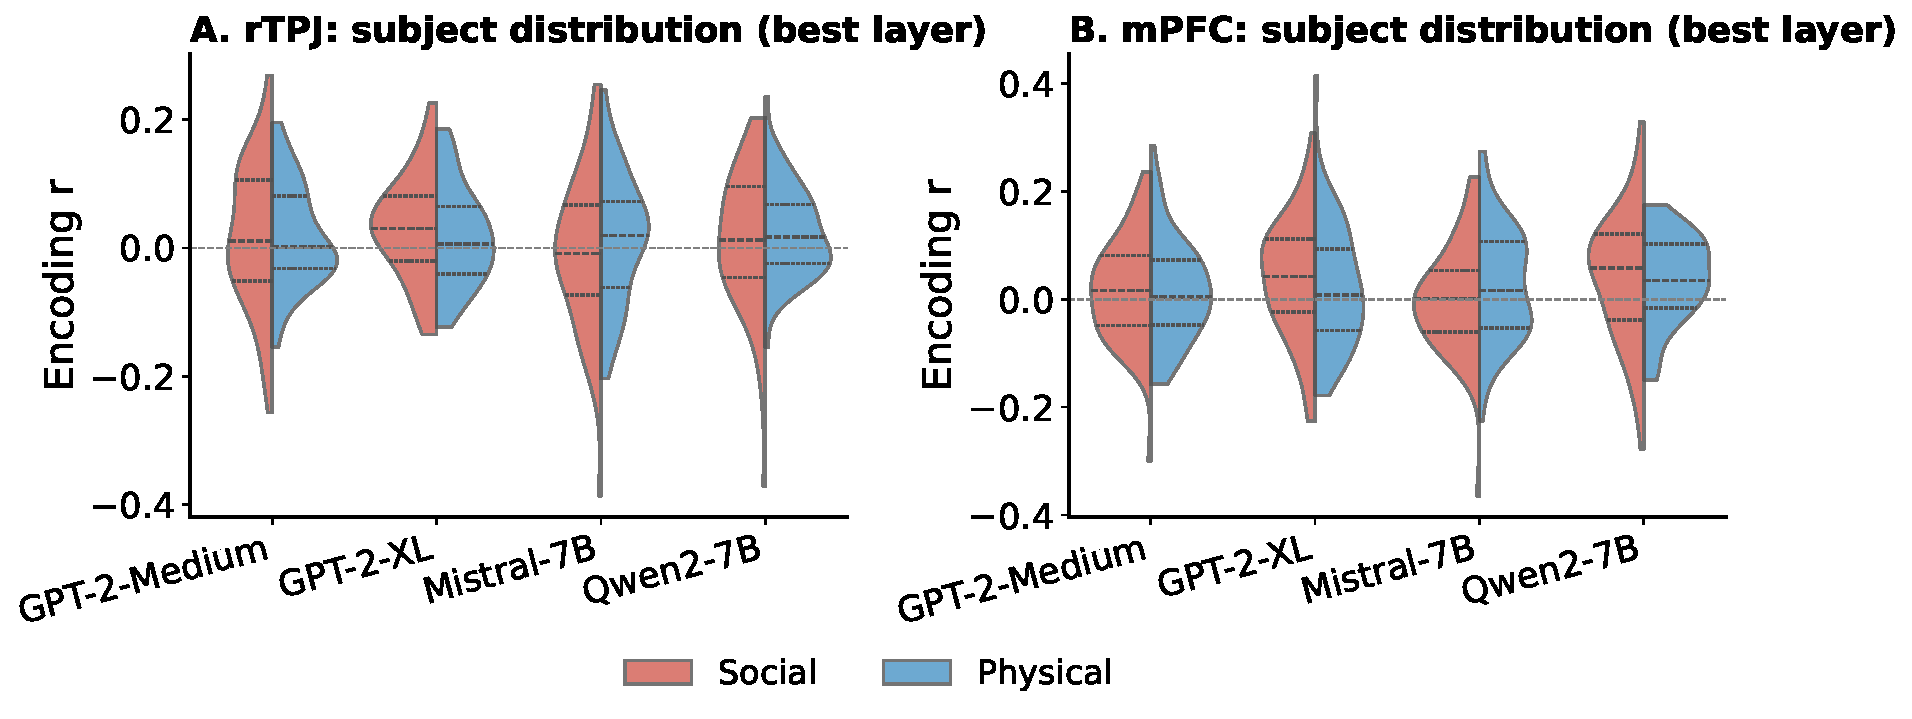
\includegraphics[width=\linewidth]{fig03_violin_encoding.pdf}
\caption{Subject-level encoding $r$ distributions at each model's best layer, split by condition. (A) rTPJ, (B) mPFC. Violins span the N=58 subjects; dashed horizontal line marks $r=0$. Median encoding is positive but small for all models, with broad across-subject variability exceeding the condition difference.}
\label{fig:enc-violin}
\end{figure}

\subsection{Attention Sparsity: Architecture-Specific Patterns}
\label{sec:attention-sparsity-results}

Attention sparsity analysis found moderately concentrated attention across all models, with small but consistent condition differences (Fig.~\ref{fig:attention}). Across the three complementary metrics (Table~\ref{tab:sparsity}), Mistral-7B stood out with the highest Gini (0.768 social vs.\ 0.752 physical), the lowest entropy (0.499 social vs.\ 0.525 physical), and the highest top-5 concentration (0.568 social vs.\ 0.538 physical), indicating that roughly 57\% of the attention mass lands on just five tokens. In contrast, GPT-2-XL showed essentially uniform entropy (0.69) and the lowest top-5 concentration (0.32--0.36), consistent with its more diffuse attention pattern visible in the per-head heatmaps.

\begin{table}[t]
\centering
\caption{Attention sparsity by model and condition (S = social, P = physical).}
\label{tab:sparsity}
\vskip 0.05in
\small
\setlength{\tabcolsep}{3pt}
\begin{tabular}{lcccccc}
\toprule
 & \multicolumn{2}{c}{Gini} & \multicolumn{2}{c}{Entropy} & \multicolumn{2}{c}{Top-5} \\
Model & S & P & S & P & S & P \\
\midrule
GPT-2-Medium & 0.661 & 0.648 & 0.664 & 0.702 & 0.393 & 0.351 \\
GPT-2-XL     & 0.672 & 0.675 & 0.688 & 0.714 & 0.358 & 0.323 \\
Mistral-7B   & \textbf{0.768} & \textbf{0.752} & \textbf{0.499} & \textbf{0.525} & \textbf{0.568} & \textbf{0.538} \\
Qwen2-7B     & 0.672 & 0.653 & 0.672 & 0.699 & 0.380 & 0.349 \\
\bottomrule
\end{tabular}
\end{table}

All four models had slightly higher sparsity for social than physical narratives by at least two of the three metrics, but effect sizes were small (average $\Delta$Gini $\approx 0.01$). Across all models and both conditions, the fraction of heads classified as ``sparse'' (Gini~$>0.5$) exceeded 80\%, rising to 96.1\% for Mistral-7B social, suggesting that the vast majority of heads implement some form of concentrated selection rather than diffuse averaging. Layer-by-head heatmaps indicated that sparsity patterns also varied across architectures: GPT-2 models have more uniform sparsity across heads, while Mistral-7B and Qwen2-7B exhibit greater head-level variability, with some heads showing highly concentrated attention (Gini $> 0.9$) and others showing diffuse patterns (Gini $< 0.5$).

\begin{figure}[t]
\centering
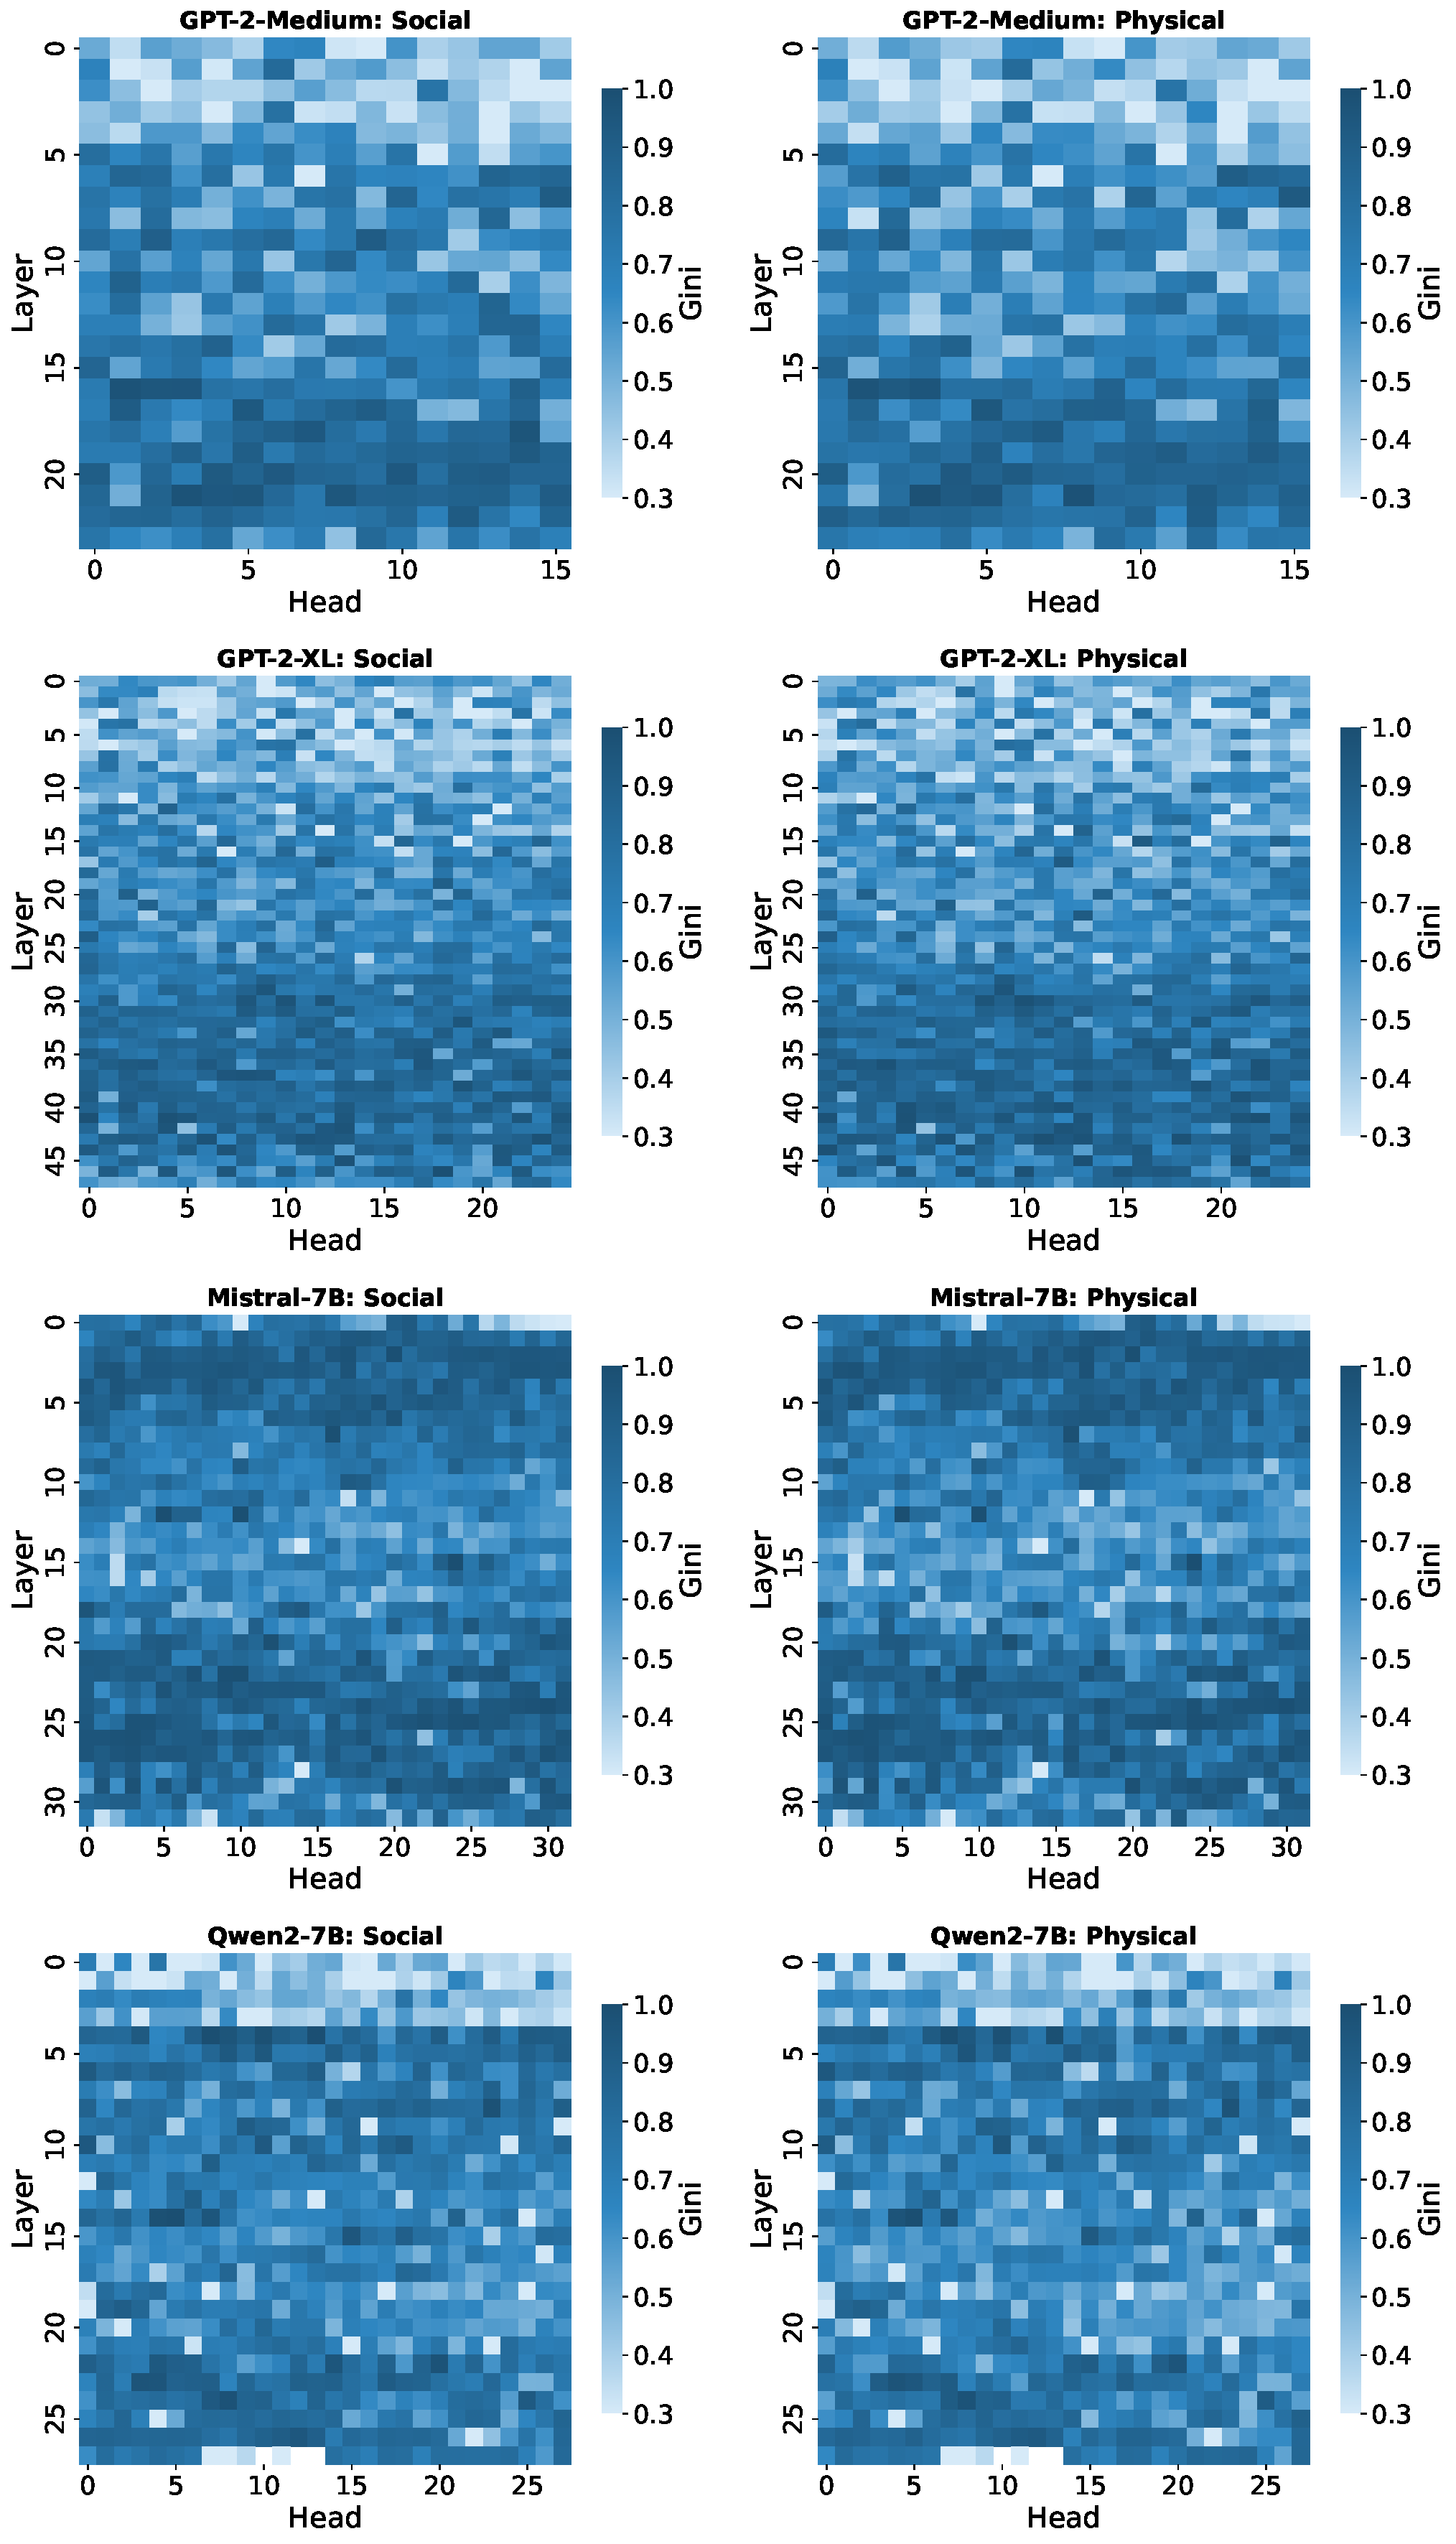
\includegraphics[width=\linewidth]{fig03_attention_heatmaps.pdf}
\caption{Attention sparsity heatmaps showing Gini coefficient per layer (rows) and head (columns) for each model. Left: social condition; right: physical condition. Darker colors indicate higher sparsity.}
\label{fig:attention}
\end{figure}

\subsection{Causal Head Ablation: ToM Circuits Are Small}
\label{sec:ablation}

Zero-ablating individual attention heads showed that mental-state word prediction depends on a small subset of heads rather than being diffusely encoded (Table~\ref{tab:ablation}). For GPT-2-Medium, a single head (layer 6, head 1) carried a causal effect of $\Delta = 0.94$ logits, nearly 25\% of the model's entire baseline logit gap (3.81). Mistral-7B's most critical head was located at the very first layer (layer 0, head 29) with $\Delta = 0.50$ (13\% of baseline), while GPT-2-XL and Qwen2-7B produced broader but more moderate maxima of 0.22 and 0.34, with top heads distributed across middle and upper layers. The four models also differed markedly in their \textit{mean} ablation effect: GPT-2 variants and Mistral-7B yielded near-zero or slightly positive means (consistent with most heads being weakly helpful), while Qwen2-7B produced a \emph{negative} mean ($-0.08$), indicating that on average ablating one of its heads \emph{improves} the target--control logit gap and only a small critical subset carries the positive signal. Consistent with prior reports of sparse, identifiable circuits in transformer models \cite{wang2022interpretability, conmy2023towards}, the top-5\% critical heads were predominantly middle-layer (41--68\% at 33--67\% relative depth) with a consistent secondary contribution from early layers (23--33\%). Late-layer contributions were generally smaller ($8$--$11\%$ for GPT-2 and Mistral) but substantial in Qwen2-7B (26\%), indicating that some architectures perform mental-state integration deeper in the network than others. The overall picture is one of a distributed circuit concentrated in middle layers but with genuinely causal heads at every depth.

\begin{table}[t]
\centering
\caption{Causal head ablation summary. Max is the single largest per-head drop in target-word logit; critical heads are those $\geq$95th percentile.}
\label{tab:ablation}
\vskip 0.05in
\footnotesize
\setlength{\tabcolsep}{4pt}
\begin{tabular}{lcccc}
\toprule
Model & Base & Max & Mean & N crit. \\
\midrule
GPT-2-Med.  & 3.81 & \textbf{0.94} & $+0.013$ & 20/384 \\
GPT-2-XL    & 2.33 & 0.22 & $+0.000$ & 60/1200 \\
Mistral-7B  & 3.90 & 0.50 & $+0.008$ & 57/1024 \\
Qwen2-7B    & 3.41 & 0.34 & $-0.081$ & 46/784 \\
\bottomrule
\end{tabular}
\end{table}

\section{Discussion}

\subsection{Behavioral Success Without Representational Alignment}

Our findings expose a dissociation between behavioral competence and neural alignment. 7B transformer models solve explicit ToM items at 75--83\% accuracy, and all four models we tested readily distinguish social from physical descriptions of identical visual events (81--88\% probing accuracy), yet their internal representations align only weakly with human brain activity during the same task ($r \approx 0.03$--$0.04$). Transformers and brains may thus solve similar ToM-related tasks through fundamentally different computational strategies.

The weak encoding performance should be interpreted relative to the noise ceiling. With ISC-based upper bounds of 0.16--0.25, the best encoding correlations ($r \approx 0.04$) achieve roughly 15--20\% of the ceiling. This is substantially lower than encoding results reported for language comprehension, where models can explain 20--50\% of the neural variance \cite{schrimpf2021neural, caucheteux2022brains, goldstein2022shared}. The gap suggests that social cognition involves computational principles not well captured by current language model architectures.

\subsection{Early Representational Divergence}

The probing results show that social--physical distinctions emerge in the earliest layers (layers 2--3 for Mistral-7B and Qwen2-7B), consistent with lexical-level differences between the conditions. This early divergence contrasts with the brain's ToM processing, which involves higher-order inference about agents' beliefs and intentions beyond word-level features. The models may classify content based on vocabulary signatures (mental-state words vs.\ geometric terms) rather than mentalizing computations, explaining why behavioral classification succeeds while deeper representational alignment remains weak.

\subsection{Model Scale and Alignment Trends}

The four models span roughly 20$\times$ in parameter count (355M to 7B), providing a small but informative window into scaling effects. Behavioral ToM accuracy tracks parameter count cleanly: 7B models (83.3\% and 75.0\% overall) nearly double the performance of the GPT-2 variants ($\sim$50\%). Brain-model encoding alignment, however, shows no such monotonic trend: the best mPFC correlation is only marginally higher for Qwen2-7B ($r = 0.039$) than for GPT-2-XL ($r = 0.037$) despite nearly a 5$\times$ gap in parameter count, and GPT-2-XL outperforms both 7B models on rTPJ ($r = 0.031$). This flat-to-weak relationship between scale and brain alignment, in sharp contrast to the near-doubling of behavioral accuracy from GPT-2 to 7B, echoes concerns raised in the wider scaling-law literature: parameter count improves task performance more reliably than it improves representational plausibility. It also constrains the interpretation of larger models (e.g., GPT-4) that solve textbook ToM tasks \cite{kosinski2024evaluating, strachan2024testing}: impressive behavioral performance need not imply brain-like mechanisms.

\subsection{Layer Trajectories and the Missing Middle}

In language comprehension studies, encoding peaks typically occur in the \textit{middle} layers of transformer models (around 50--70\% depth), reflecting a hierarchy from lexical to compositional to semantic processing \cite{caucheteux2022brains, schrimpf2021neural}. Our data show an inconsistent picture: best-encoding layers for mPFC range from layer 9 of GPT-2-Medium (38\% depth) to layer 28 of GPT-2-XL (58\%) to layer 22 of Qwen2-7B (79\%), and probing accuracy peaks even earlier (layers 2--3 for the 7B models). That probing and brain-encoding peaks do not co-locate on the layer axis suggests that the features the probe relies on (likely lexical) and the features the brain activity reflects (presumably integrative) live in different parts of the network. This is a mechanistic view of the behavior/alignment dissociation and motivates future work on intermediate representations between linear-probe accessible features and higher-order social inference.

\subsection{Implications for AI Safety and Evaluation}

Our results caution against using behavioral ToM benchmarks as evidence for genuine social understanding in AI systems. The dissociation between behavioral performance and representational alignment underscores that passing ToM tasks does not imply human-like mentalizing mechanisms. This finding has implications for AI safety: systems that appear to understand social situations may rely on fundamentally different, and potentially brittle, computational strategies.

\subsection{Limitations and Future Directions}

Several limitations should be noted. First, our encoding model uses linear mapping (ridge regression), which may underestimate alignment detectable through nonlinear methods. Second, we used atlas-based ROIs rather than individually localized regions, which introduces spatial imprecision despite MNI normalization. Third, the raw BOLD data were not processed through fMRIPrep, potentially reducing signal quality. Fourth, only four of six planned models could be analyzed due to compatibility issues. Fifth, our behavioral ToM benchmark (24 items) is small; larger, contamination-controlled benchmarks would strengthen the scaling conclusions. Sixth, the causal ablation used four narrative-derived prompts; broader prompt sets would better characterize circuit generality, and early-layer findings (e.g., the dominant layer-0 head in Mistral-7B) should be interpreted with care since layer-0 heads often specialize in position- or BOS-token attention that is structurally, rather than semantically, critical. Future work should employ fMRIPrep-processed data with individually localized ROIs, nonlinear encoding approaches, larger and more diverse behavioral/ablation sets, and larger model families including multimodal models that can process visual ToM stimuli directly.

\subsection{Conclusion}

This study provides modality-matched evidence that 7B-scale transformer language models solve classic Theory of Mind items at 75--83\% accuracy. Linear probes across all four models we tested further distinguish social from physical narratives in their hidden states (81--88\% accuracy). Yet despite this behavioral and representational competence, the models' internal states align only weakly ($r \approx 0.04$, 15--20\% of the ISC noise ceiling) with the human brain's social cognition network. Causal head ablation on narrative-target word prediction further identifies a distributed circuit of a few dozen heads concentrated in middle layers, providing a mechanistic anchor for the models' behavioral competence. The dissociation between behavioral success and representational alignment suggests that current LLMs achieve ToM-like performance through computational strategies fundamentally different from human mentalizing. For cognitive science, these results indicate that behavioral similarity should not be taken as evidence for mechanistic similarity, a principle with broad implications for evaluating AI systems' cognitive capabilities.

\section*{Code Availability}

All analysis code (fMRI preprocessing, LLM feature extraction, encoding models, probing classifiers, attention sparsity, and causal head ablation) is publicly available at \url{https://anonymous.4open.science/r/attention-tom-brain-transformer-F4FC}.

\section*{Acknowledgment}

Data were provided by the Narratives collection \cite{nastase2021narratives} (OpenNeuro ds002345). We thank the Princeton Neuroscience Institute for data collection and sharing.

\begin{thebibliography}{00}

\bibitem{frith2006neural} C. D. Frith and U. Frith, ``The neural basis of mentalizing,'' \textit{Neuron}, vol. 50, no. 4, pp. 531--534, 2006.

\bibitem{saxe2013people} R. Saxe, ``The new puzzle of Theory of Mind development,'' in \textit{Navigating the Social World}, A. Banaji and S. Gelman, Eds. Oxford Univ. Press, 2013.

\bibitem{soutschek2025causal} A. Soutschek et al., ``Causal role of the temporo-parietal junction in Theory of Mind,'' \textit{Neurosci. Biobehav. Rev.}, 2025.

\bibitem{amodio2006meeting} D. M. Amodio and C. D. Frith, ``Meeting of minds: the medial frontal cortex and social cognition,'' \textit{Nat. Rev. Neurosci.}, vol. 7, pp. 268--277, 2006.

\bibitem{allison2000social} T. Allison, A. Puce, and G. McCarthy, ``Social perception from visual cues: role of the STS region,'' \textit{Trends Cogn. Sci.}, vol. 4, no. 7, pp. 267--278, 2000.

\bibitem{mar2011neural} R. A. Mar, ``The neural bases of social cognition and story comprehension,'' \textit{Annu. Rev. Psychol.}, vol. 62, pp. 103--134, 2011.

\bibitem{kosinski2024evaluating} M. Kosinski, ``Evaluating large language models in Theory of Mind tasks,'' \textit{arXiv:2302.02083}, 2024.

\bibitem{ullman2023large} T. Ullman, ``Large language models fail on trivial alterations to Theory-of-Mind tasks,'' \textit{arXiv:2302.08399}, 2023.

\bibitem{shapira2024clever} N. Shapira et al., ``Clever Hans or neural Theory of Mind?,'' in \textit{Proc. EACL}, 2024.

\bibitem{strachan2024testing} J. W. A. Strachan et al., ``Testing Theory of Mind in large language models and humans,'' \textit{Nat. Hum. Behav.}, vol. 8, pp. 1285--1295, 2024.

\bibitem{chen2024tombench} Z. Chen et al., ``ToMBench: Benchmarking Theory of Mind in large language models,'' in \textit{Proc. ACL}, 2024.

\bibitem{wilf2024think} N. Wilf et al., ``Think twice: Perspective-taking improves large language models' Theory-of-Mind capabilities,'' in \textit{Proc. ACL}, 2024.

\bibitem{sap2022neural} M. Sap et al., ``Neural Theory-of-Mind? On the limits of social intelligence in large LMs,'' in \textit{Proc. EMNLP}, 2022.

\bibitem{marcus2023large} G. Marcus, ``Large language models and the limits of understanding,'' \textit{AI Mag.}, 2023.

\bibitem{khaligh2014deep} S. A. Khaligh-Razavi and N. Kriegeskorte, ``Deep supervised, but not unsupervised, models may explain IT cortical representation,'' \textit{PLoS Comput. Biol.}, vol. 10, e1003915, 2014.

\bibitem{schrimpf2021neural} M. Schrimpf et al., ``The neural architecture of language: Integrative modeling converges on predictive processing,'' \textit{Proc. Natl. Acad. Sci.}, vol. 118, e2105646118, 2021.

\bibitem{caucheteux2022brains} C. Caucheteux and J.-R. King, ``Brains and algorithms partially converge in natural language processing,'' \textit{Commun. Biol.}, vol. 5, 134, 2022.

\bibitem{goldstein2022shared} A. Goldstein et al., ``Shared computational principles for language processing in humans and deep language models,'' \textit{Nat. Neurosci.}, vol. 25, pp. 369--380, 2022.

\bibitem{nastase2021narratives} S. A. Nastase et al., ``The `Narratives' fMRI dataset for evaluating models of naturalistic language comprehension,'' \textit{Sci. Data}, vol. 8, 250, 2021.

\bibitem{schurz2014fractionating} M. Schurz et al., ``Fractionating Theory of Mind: A meta-analysis of functional brain imaging studies,'' \textit{Neurosci. Biobehav. Rev.}, vol. 42, pp. 9--34, 2014.

\bibitem{kriegeskorte2008representational} N. Kriegeskorte, M. Mur, and P. Bandettini, ``Representational similarity analysis,'' \textit{Front. Syst. Neurosci.}, vol. 2, 4, 2008.

\bibitem{elhage2021mathematical} N. Elhage et al., ``A mathematical framework for transformer circuits,'' \textit{Transformer Circuits Thread}, Anthropic, 2021.

\bibitem{wang2022interpretability} K. Wang et al., ``Interpretability in the wild: a circuit for indirect object identification in GPT-2 small,'' in \textit{Proc. ICLR}, 2022.

\bibitem{conmy2023towards} A. Conmy et al., ``Towards automated circuit discovery for mechanistic interpretability,'' in \textit{Proc. NeurIPS}, 2023.

\bibitem{wolf2020transformers} T. Wolf et al., ``Transformers: State-of-the-art natural language processing,'' in \textit{Proc. EMNLP: System Demonstrations}, 2020, pp. 38--45.

\bibitem{hoyer2004non} P. O. Hoyer, ``Non-negative matrix factorization with sparseness constraints,'' \textit{J. Mach. Learn. Res.}, vol. 5, pp. 1457--1469, 2004.

\end{thebibliography}

\end{document}
